%#BIBTEX upbibtex abst
\synctex=1
%%%%%%%%%%%%%%%%%%%%%%%%%%%%%%%%%%%%%%%%%%%%%%%%
%   土木学会応用力学論文集マニュアル           %
%      applmech.sty を勝手に改編               %
%%%%%%%%%%%%%%%%%%%%%%%%%%%%%%%%%%%%%%%%%%%%%%%%
\documentclass[twocolumn,uplatex]{jsarticle}  %ASCII
\def\gtfam{applmech}
\usepackage{applm-2e}
\usepackage{here}
\usepackage[dvipdfmx]{xcolor}
\usepackage{amsmath,amssymb,bm}
\usepackage{amsmath}
\usepackage[dvipdfmx]{graphicx}
\usepackage[ruled,vlined]{algorithm2e}
\newcommand\figref[1]{{{図}-\ref{fig:#1}}}
\newcommand\tabref[1]{{{表}\ref{tab:#1}}}
\renewcommand\eqref[1]{式(\ref{eq:#1})}
\renewcommand{\figurename}{\mc{図-}}
\renewcommand{\thesubsection}{(\arabic{subsection})}
\newenvironment{jalgorithm}[1][htb]
  {\renewcommand{\algorithmcfname}{アルゴリズム}% Update algorithm name
   \begin{algorithm}[#1]%
  }{\end{algorithm}}
\newcommand{\bs}[1]{\boldsymbol{#1}}
\newcommand{\ya}[1]{\overrightarrow{#1}}
%\usepackage{showkeys}
% 査読が通って,搭載可となった場合には,次の行をアンコメントしてください。
%\AcceptedPaper %<<<意味不明
%%%%%%%%%%%%%%%%%%%%%%%%%%%%%%%%%%%%%%%%%%%%%%%%%%%%%%
 \usepackage[dvipdfm,bookmarks=false,bookmarksnumbered=false,implicit=false,%
 hyperindex=false,plainpages=false,%
 %pdftitle={京都大学大学院社会基盤工学専攻},%
 %pdfsubject={},%
 pdfauthor={藤井遥},%
 pdfkeywords={put, about, Four key words}]{hyperref}
%%%%%%%%%%%%%%%%%%%%%%%%%%%%%%%%%%%%%%%%%%%%%
%
%\volumenumber{}
\pubyear{2026}
\title{{変分法に基づく改良型PIC/FLIPによる\\3次元流体解析の境界条件処理に関する研究}}
\endtitle{
  Boundary condition treatment in three-dimensional fluid analysis 
  \\using an improved variational PIC/FLIP Method
}
\author{岡本 連太郎\thanks{応用力学講座}}
\endauthor{Okamoto Retnaro}
%\receivedate{田村武教授、角哲也准教授、小林俊一助教、吉川仁助教}
% \vspace{-5mm}

%section subsectionの前後を調整
\makeatletter %
  \renewcommand{\section}{%
    \@startsection{section}{1}{\z@}%
    {0.3\Cvs}{0.2\Cvs}%
    {\normalfont\large\headfont\raggedright}}

  \renewcommand{\subsection}{\@startsection{subsection}{2}{\z@}%
    {\z@}{\if@slide .4\Cvs \else \z@ \fi}%
%    {1\Cvs}{1\Cvs}
    {\normalfont\normalsize\headfont}}

\makeatother
\setlength{\abovedisplayskip}{1pt}
\setlength{\belowdisplayskip}{1pt}
\setlength{\abovecaptionskip}{0pt}
\setlength{\textfloatsep}{1pt}
\setlength{\intextsep}{1pt}
\begin{document}


\maketitle
\thispagestyle{empty}
\pagestyle{empty}
\section{序論}
% \vspace{-2mm}.
流体の解析手法は格子法と粒子法に大別される.
格子法と粒子法のハイブリッド手法であるPIC/FLIP(Particle-In-Cell/Fluid-Implicit-Particle)\cite{10.1145/1186822.1073298}を改良することが本研究の目的である.
PIC/FLIPは,流体を表す移動可能な流体粒子と,空間に設定された格子上の点(ノード)を用いる手法である.
ノードで更新された物理量を流体粒子に補間し,その物理量により流体粒子を動かすことで流体の運動を表現する.

PIC/FLIPの利点として,格子法の安定性と粒子法の自由表面追跡能力を兼ね備えていることが挙げられる.
しかし,PIC/FLIPには以下のような課題がある.
まず,非圧縮性条件を\(\nabla \cdot \boldsymbol{v}=0\)で定式化した場合,流体領域のトポロジーが変化するようなセルで非物理的に圧力が上昇する.
次に,流体粒子が初期配置を維持したまま移動することで,粒子が存在しない空のセルが発生する問題がある.
本研究では,これらの課題を解決するために,変分法に基づく圧力Poisson方程式の導出と,
Smoothed Particle Hydrodynamics(SPH)\cite{gingold1977}の圧力勾配モデルの導入を提案する.

\section{数値計算法}
\subsection{GIMPを用いた補間}
流体粒子からノードへの物理量の補間に,Generalized Interpolation Material Point Method(GIMP)\cite{Bardenhagen2004GIMP}
を用いることで,流体粒子がセルを跨いで移動した際の不連続な補間値の変化を抑制する(\figref{uniformGIMP}).

\begin{figure}[htbp]
  \begin{center}
    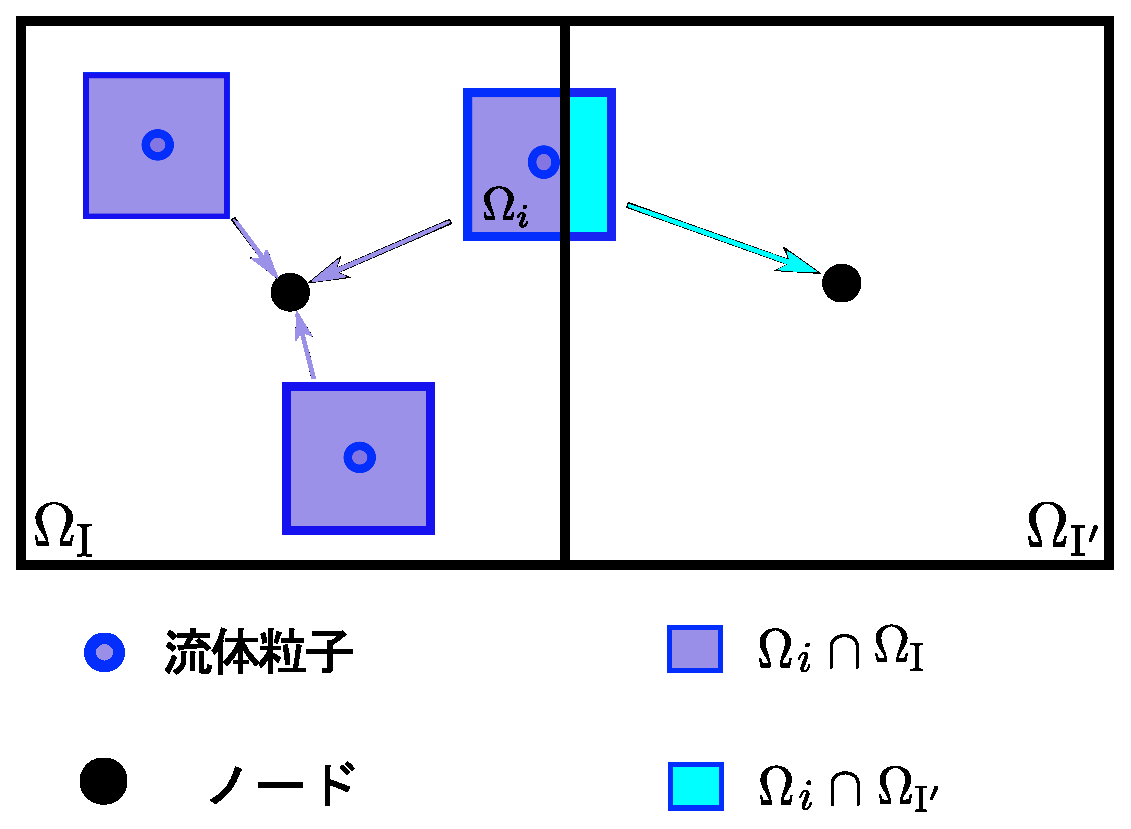
\includegraphics[scale=0.2]{eps/uniformGIMP.eps}
  \end{center}
  \caption{uniformGIMPの物理量補間}
  \label{fig:uniformGIMP}
\end{figure}
%\section{スタッガード格子}
%本研究では,スタッガード格子(図\ref{fig:staggered})を用いる.
%スタッガード格子は,速度成分を各セルの面中心に配置し,圧力をセル中心に配置する格子である.
%\vspace{0.5em}
%\begin{figure}[H]
%  \begin{center}
%    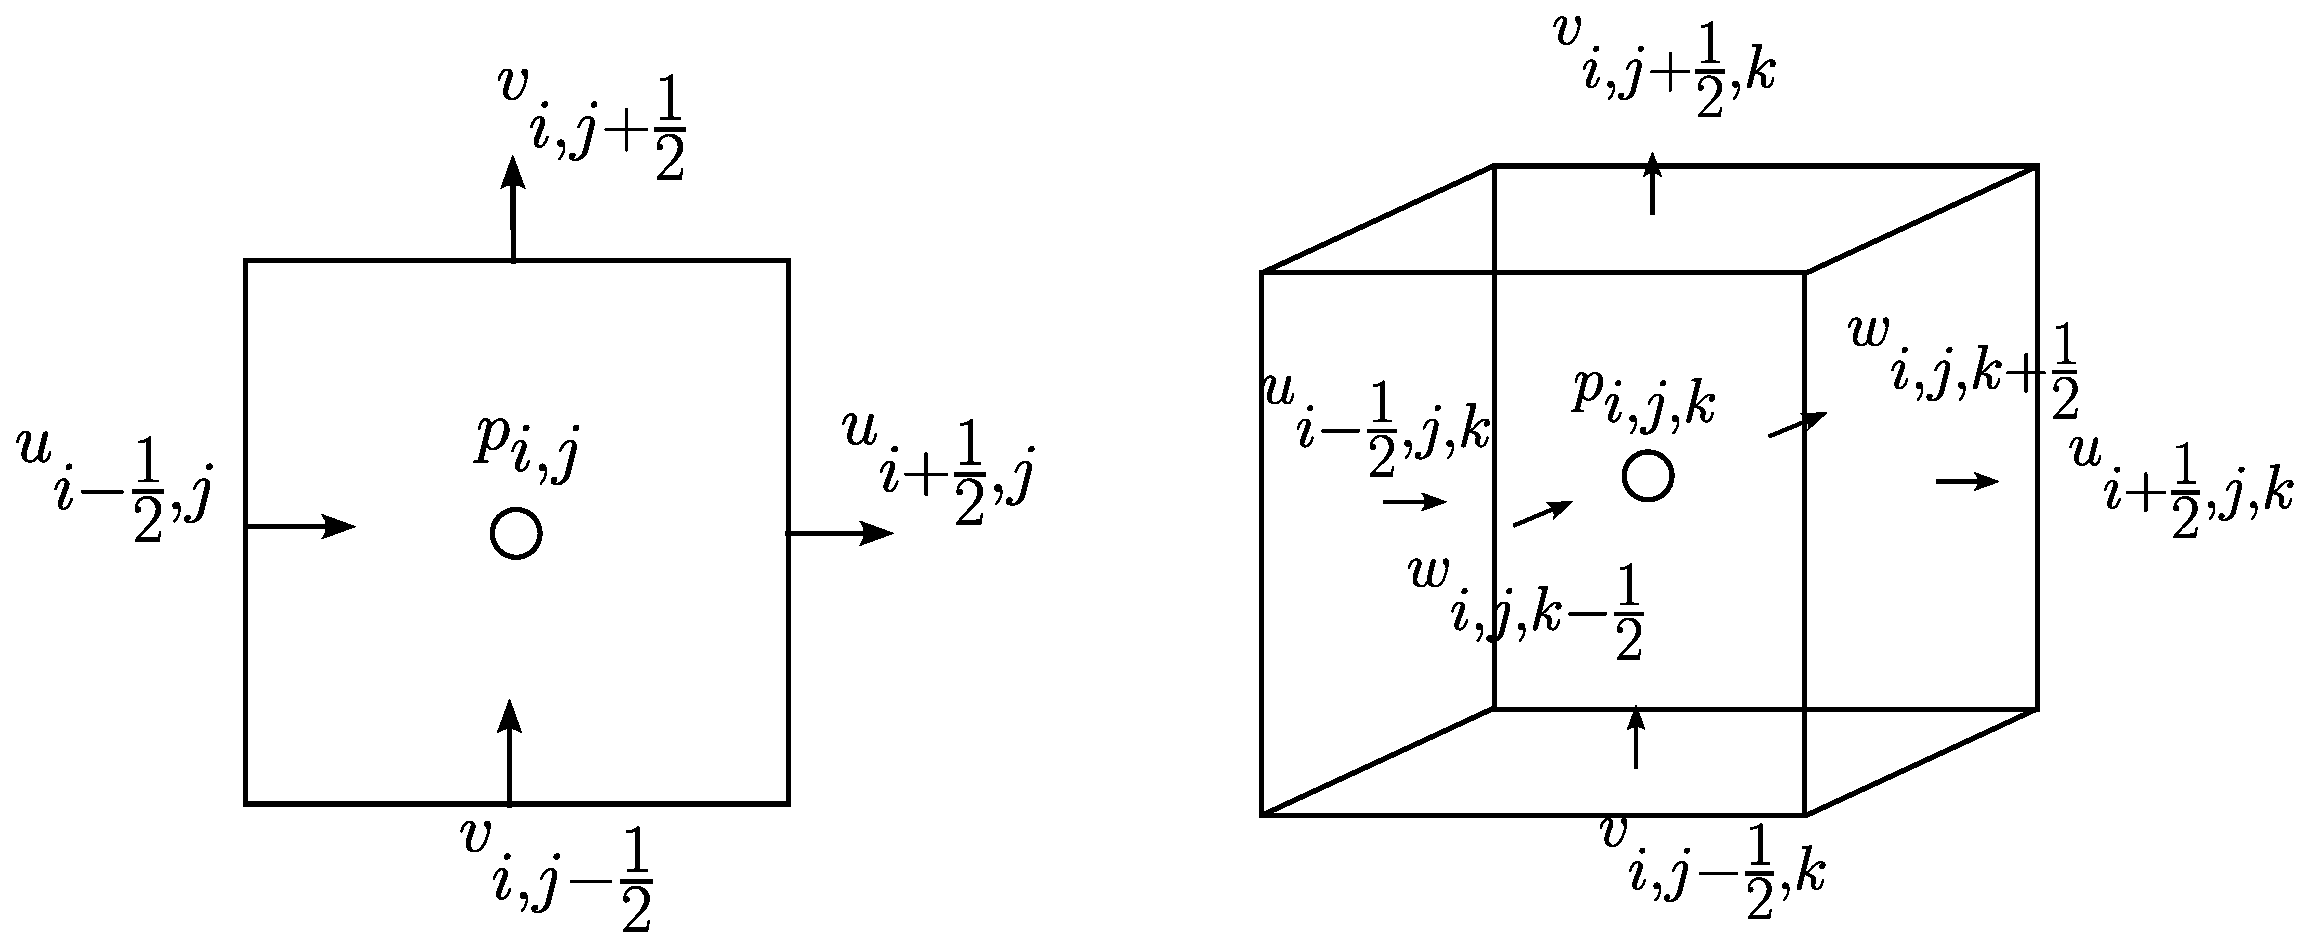
\includegraphics[scale=0.2]{eps/staggeredgrid3d.eps}
%  \end{center}
%  \caption{スタッガード格子(左:2次元,右:3次元)}
%  \label{fig:staggered}
%\end{figure}

\subsection{変分法に基づく圧力Poisson方程式の導出}
深川らによる散逸系の変分原理\cite{散逸系の変分}を参照して,
運動エネルギー,ポテンシャルエネルギー\(U\),内部エネルギー\(e\)で構成されたラグランジアン\(\mathcal{L}\)を次で与える.
\begin{equation}
  \mathcal{L}[\boldsymbol{x},\boldsymbol{v},e] = {}
  \int_{\Omega} \left(
  \frac{1}{2} \rho\, {\boldsymbol{v}}^2
  - U
  - \rho e
  \right) dV
  \label{eq:lagrangian}
\end{equation}
\(e\)は熱流がない場合の次の内部エネルギー式
\begin{equation}
  \int_{\Omega}  \left(
  \rho \frac{D e}{ D t} + \bm{t} : \bm{d}
  \right) dV = 0
  \label{eq:internalE}
\end{equation}
と,\(n+1\)ステップ目の圧力ノード\(\mathrm{I}\)の体積\(V^{n+1}_\mathrm{I}\)についての非圧縮性条件
%非圧縮性条件を
%\(\nabla \cdot \boldsymbol{v}=0\)で定式化した場合,
%流体領域のトポロジーが変化するようなセルで非物理的に圧力が上昇する.
\begin{equation}
  V^{n+1}_\mathrm{I}
  \hspace{0.2em} \leq \hspace{0.2em} V_0
  \label{eq:nocompress}
\end{equation}
を拘束条件として,\eqref{lagrangian}の作用\(\mathcal{I}\)の停留値条件を未定乗数法を用いて求める.
ただし,\(V_0\)はセル体積である.
この変分法で得られる圧力Poisson方程式により,自由表面近くのノードについて,明示的な処理をしなくても,圧力が0に近づく.
%\begin{align}
%  \sum_{d \in \{x,y,z\}} &
%  \left(
%  \frac{p^{n+1}_\mathrm{I} - p^{n+1}_{\mathrm{I}+\mathbf{e}_d}}{m^{n}_{\mathrm{I}+\frac12\mathbf{e}_d}}
%  + \frac{p^{n+1}_\mathrm{I} - p^{n+1}_{\mathrm{I}-\mathbf{e}_d}}{m^{n}_{\mathrm{I}-\frac12\mathbf{e}_d}}
%  \right)
%  \frac{V_0 (\Delta t)^2}{h^2} \notag
%  \\ \vspace{0.8em}
%                         & =
%  - \Delta t \, \left( \nabla \cdot \mathbf{u}^* \right)_\mathrm{I}
%  + \frac{V^{n}_{\mathrm{I}} - V_0}{V_0}
%  \label{eq:PPEbeta}
%\end{align}
%ただし,\(\mathbf{u}^*は粘性力・体積力で更新された中間速度,\, \mathrm{I}=(i,j,k), \,
%\mathbf{e}_x=(1,0,0), \, \mathbf{e}_y=(0,1,0), \, \mathbf{e}_z=(0,0,1)\)である.
%\(\beta\)は圧力振動を抑制するための\(\left[0,1\right]\)の定数である.
% \vspace{-2.5mm}
% \vspace{-2mm}

\subsection{SPHの圧力勾配モデル}
非圧縮性条件下のSPHの圧力勾配
\begin{align}
  \left\langle \nabla p  \right\rangle_i
   & =   \sum_{j} \left( p_j + p_i \right)\nabla W_{ij} V_j
  \label{nablap_sph}
\end{align}
を用いて,流体粒子\(i\)の速度を更新する.
ただし,壁面近くの流体粒子は,圧力勾配の壁寄与分を投影による壁境界積分を用いて評価する.
これにより,容器角部において圧力勾配をより正確に評価できる\cite{境界積分}.

\section{解析例}
本研究で用いた手法の妥当性と有効性を検証した.
\subsection{キャビティ流れ}
Ghiaらによる解析結果\cite{GHIA1982387}と,提案手法による解析結果を比較する.
\figref{cavity}で示すように,正方形容器に流体を満たし,上辺に一定流速\(U\),それ以外の辺は流速\(0\)の境界条件を課す.
定常状態の容器の中心線上の流速分布を取得する.
\begin{figure}
  \begin{center}
    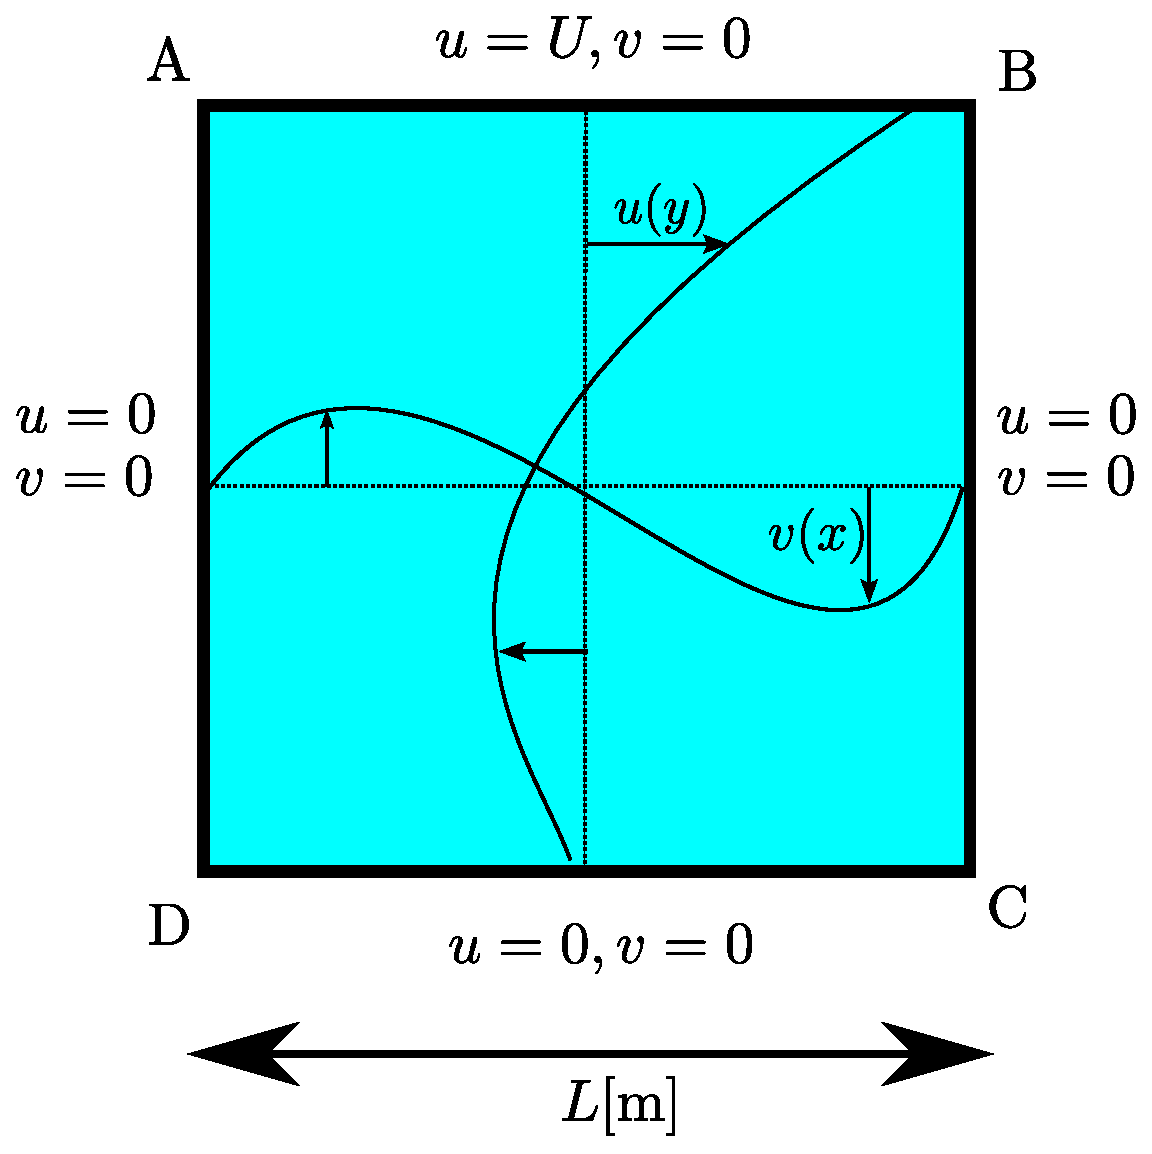
\includegraphics[scale=0.2]{eps/cavity.eps}
  \end{center}
  \caption{境界条件と測定する流速分布}
  \label{fig:cavity}
\end{figure}

\begin{figure}[H]
  \begin{center}
    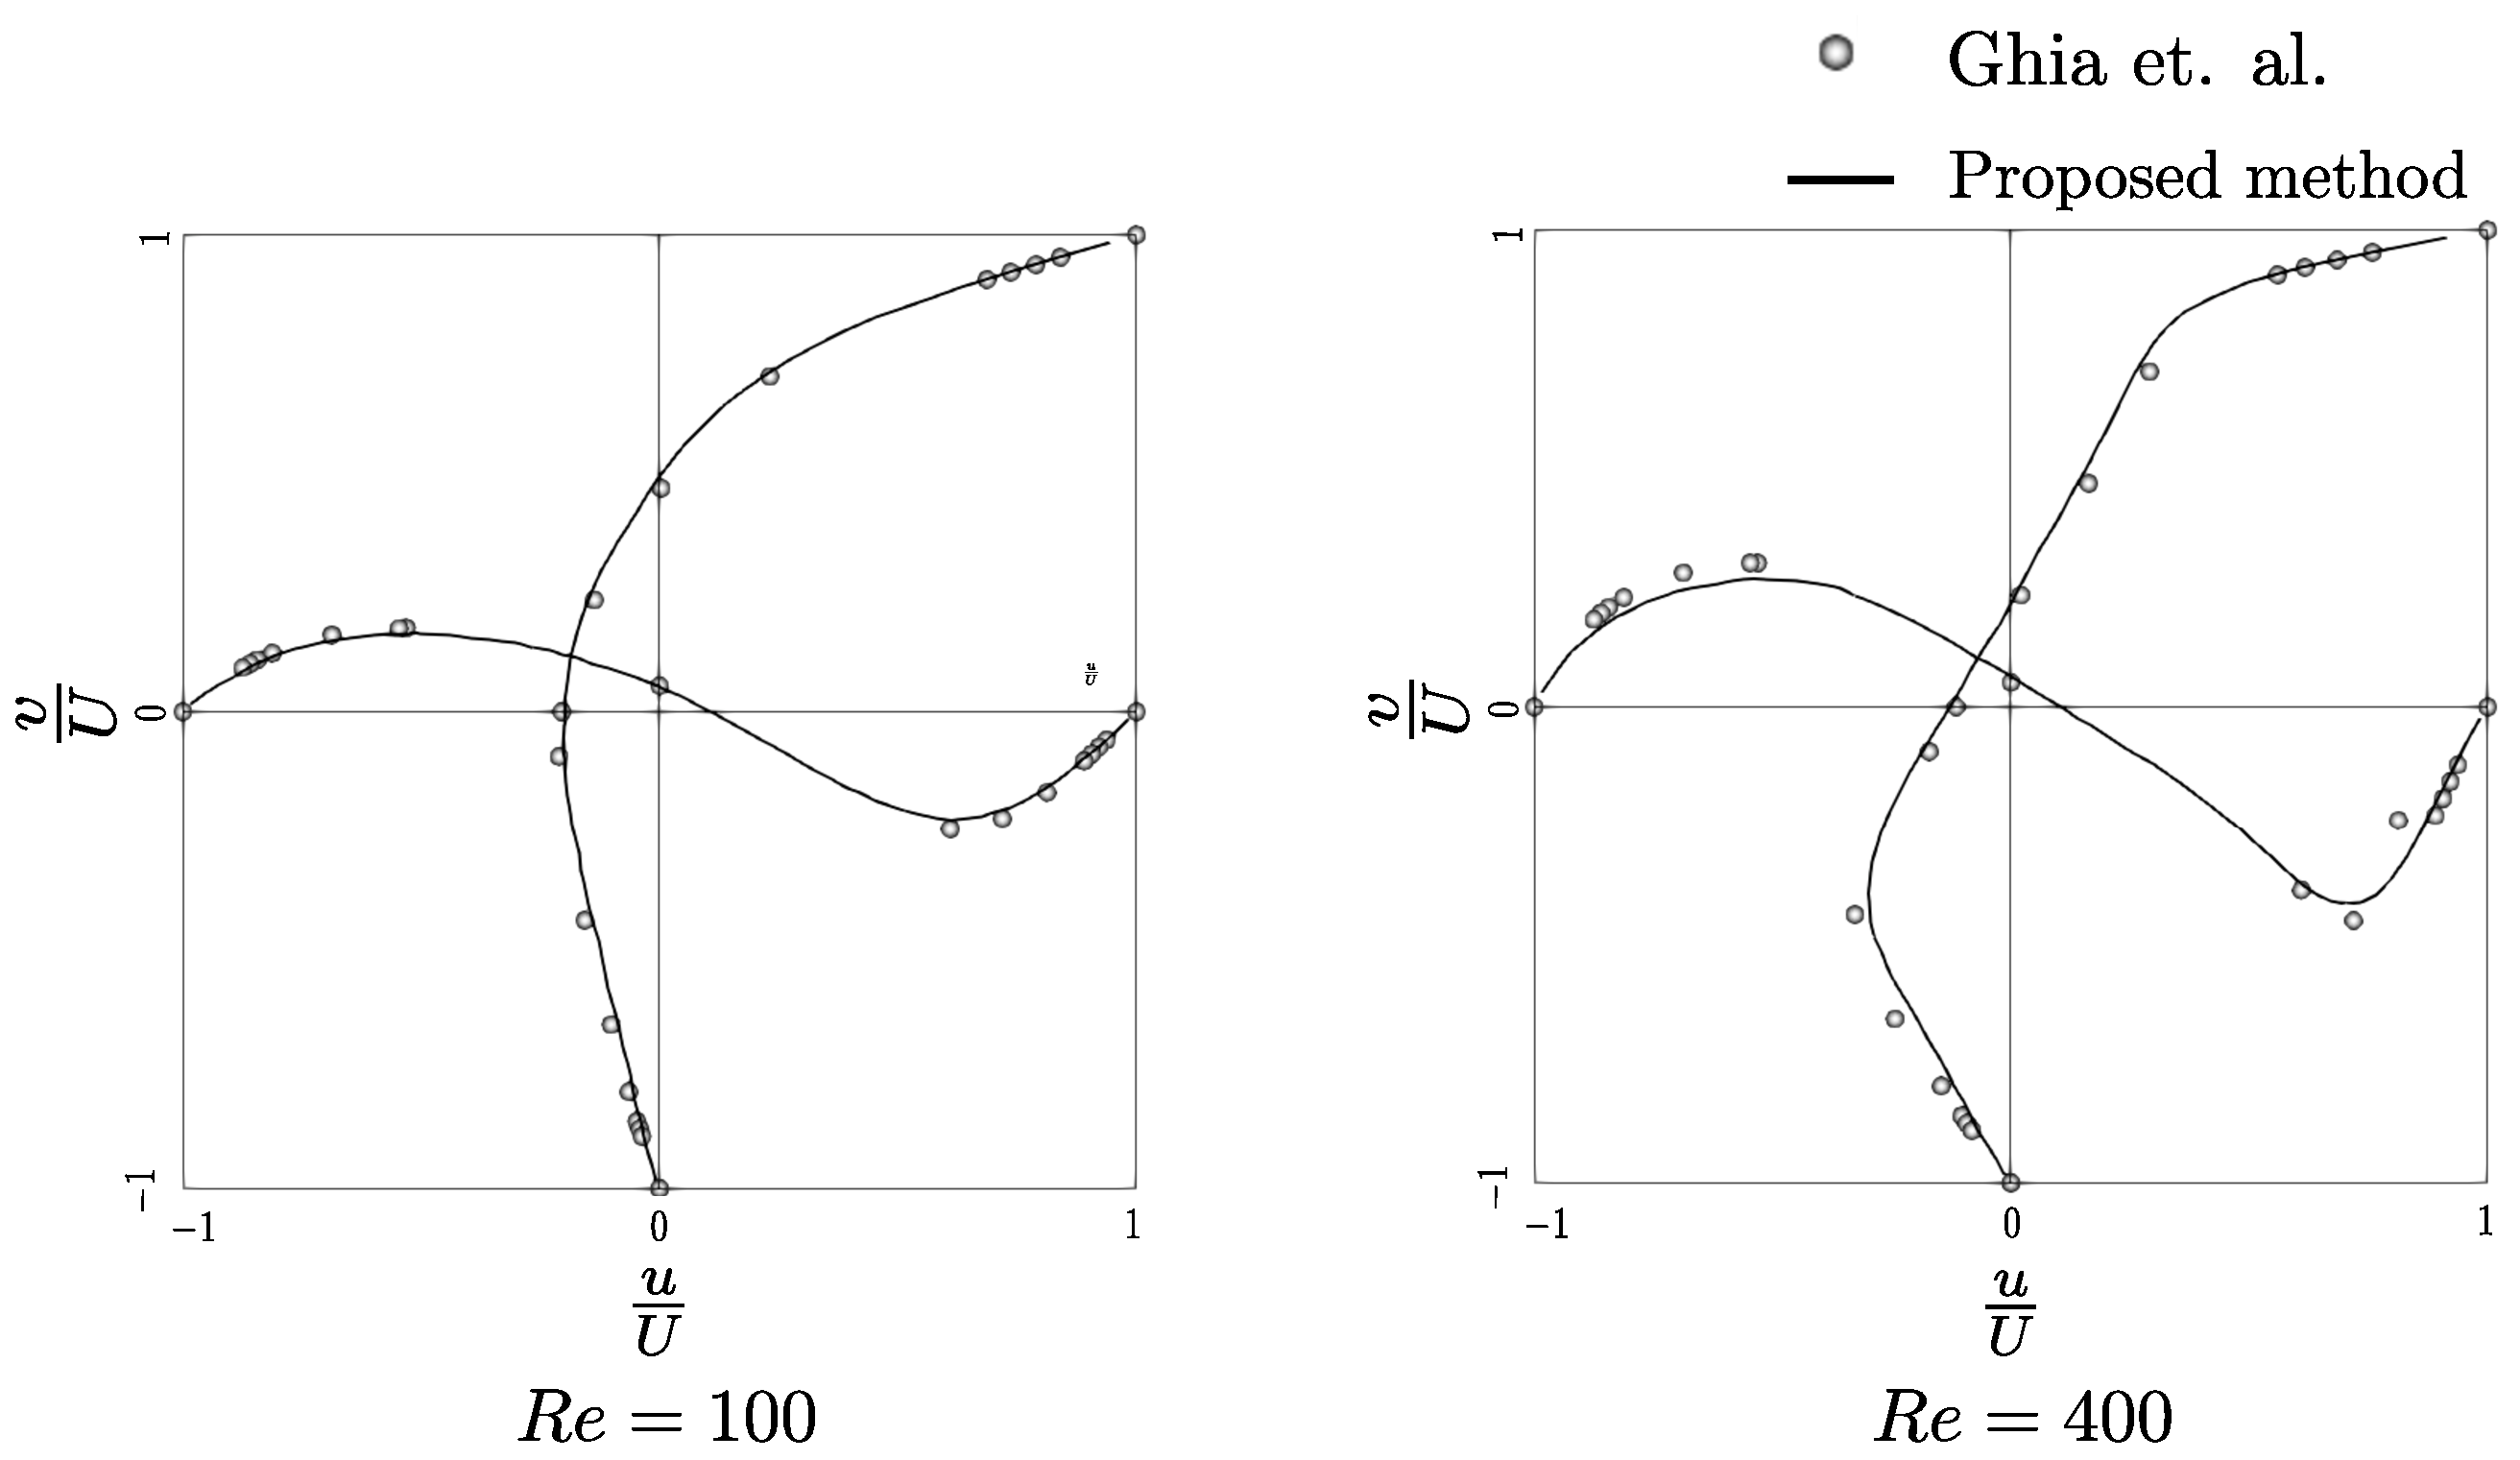
\includegraphics[scale=0.16]{eps/cavtity100400.eps}
  \end{center}
\end{figure}
\begin{figure}[H]
  \begin{center}
    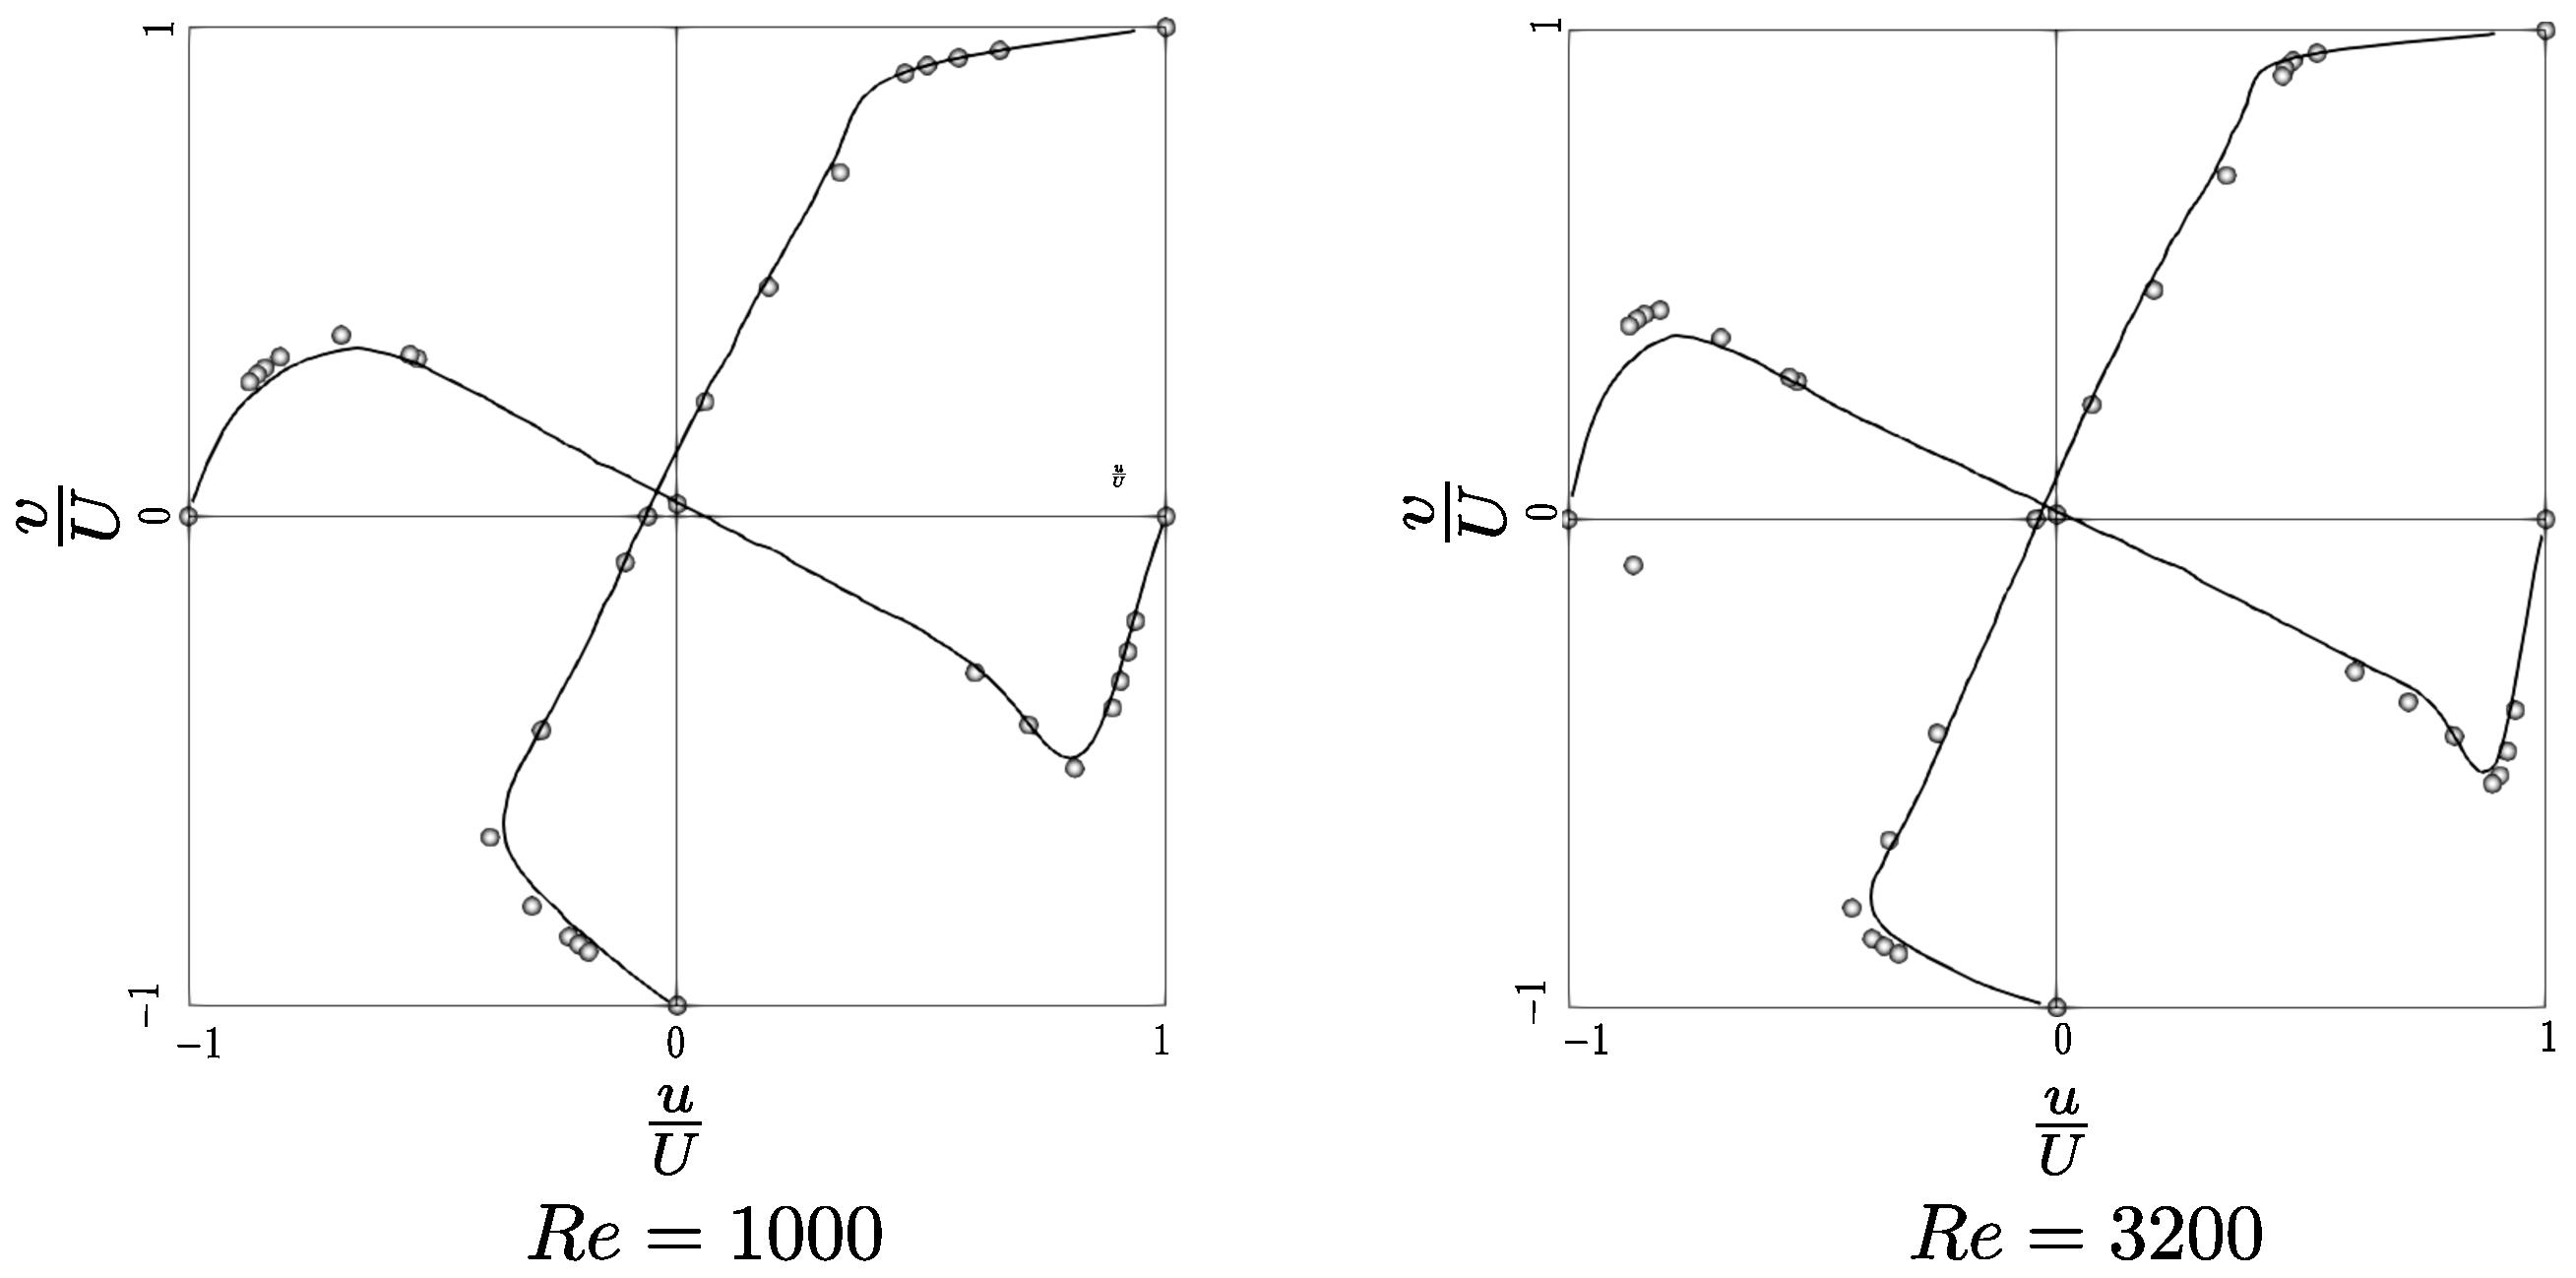
\includegraphics[scale=0.16]{eps/cavtity10003200.eps}
  \end{center}
  \caption{キャビティ流れの解析結果}
  \label{fig:cavityresult}
\end{figure}
辺BC,CD,DAの壁面近くの流速分布は,Ghiaらの解析結果よりも流速が小さくなっている.

\subsection{障害物ありダムブレイク}
Kleefsman らによるダムブレイクの実験結果\cite{KLEEFSMAN2005363}と比較する.\figref{dambreak3d}に初期状態と,障害物上に設置された圧力計測点の配置を示す.
圧力計測点における圧力推移について,実験値と本研究で提案した手法による解析結果を比較する.
\begin{figure}[H]
  \begin{center}
    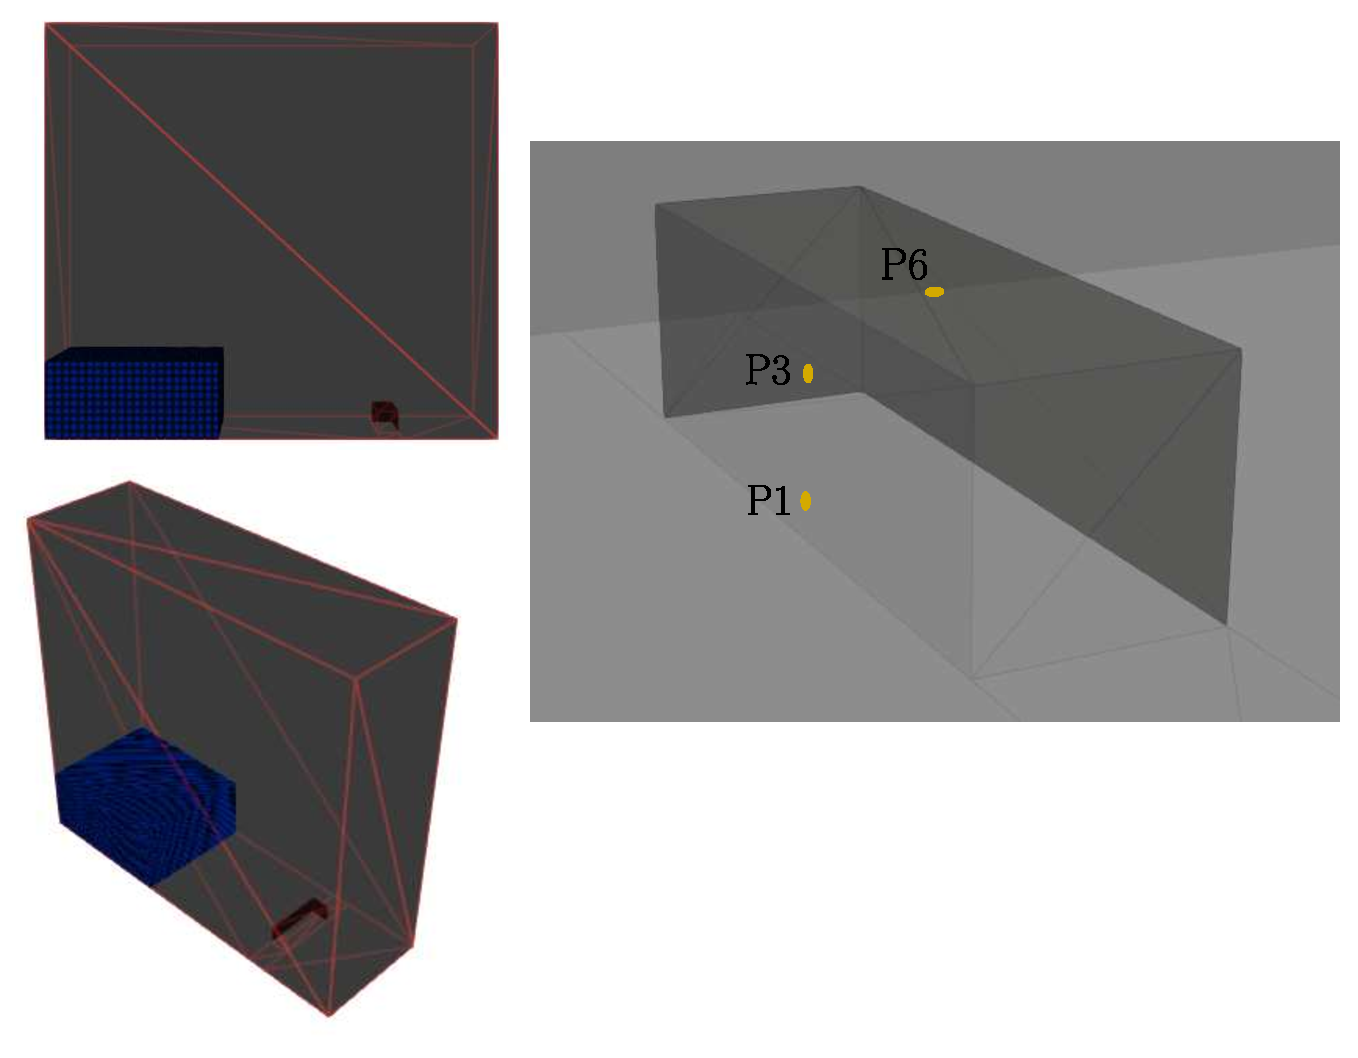
\includegraphics[scale=0.2]{eps/geo_kleefsman.eps}
  \end{center}
  \caption{初期配置と圧力測定する点P1,P3,P6}
  \label{fig:dambreak3d}
\end{figure}
\figref{output}の解析結果より,圧力推移の概形は実験値と一致する.
全体として実験値よりも圧力が大きいのは,滑りあり条件で解析したことが要因だと考える.
\begin{figure}[htbp]
  \centering
  \resizebox{0.31\linewidth}{!}{%
    \input{graph/slip_dt0001_p1.tex}
  }
  \resizebox{0.31\linewidth}{!}{%
    \input{graph/slip_dt0001_p3.tex}
  }
  \resizebox{0.31\linewidth}{!}{%
    \input{graph/slip_dt0001_p6.tex}
  }
  \caption{ダムブレイク圧力推移(左:P1,中央:P3,右:P6)}
  \label{fig:output}
\end{figure}

\section{結論}
まず,変分法により,明示的な自由表面判定を行わずに,
スタッガード格子上の非圧縮性粘性流体の支配方程式と圧力Poisson方程式を導出した.
その際,非圧縮性条件は\(\nabla \cdot \boldsymbol{v}=0\)ではなく,セル体積の不等式制約を用いた.
次に,SPHの圧力勾配モデルを導入することで,SPHの圧力勾配により流体粒子の不均一な分布を抑制した.

この提案手法を用いて,キャビティ流れ,ダムブレイクの先行研究と比較した結果,次のように考察した.
1セルあたりの流体粒子の配置数を大きくすること,圧力Poisson方程式に緩和係数を導入することが,圧力振動を抑制する効果を有する.
緩和係数の導入により,僅かな非圧縮性を許容することになり,誤差の原因になると考える.

\bibliographystyle{jsce}
\bibliography{list}

\begin{flushright}
  \vspace{-2.8mm}
  {\bf 修士論文指導教員}\\
  \vspace{1mm}
  {\bf 西藤潤准教授\\
    Abbas Khayyer准教授\\}
\end{flushright}
%\lastpagesetting

\end{document}
